% !TeX root = ../main.tex
\documentclass[./../main.tex]{subfiles}

\begin{document}

Phần này mô tả sản phẩm cuối và các luồng sau quá trình phát triển, bao gồm hình ảnh của giao diện người dùng thuộc phần client. Phần giao diện người dùng sẽ được bạn Phạm Thị Dân mô tả kỹ hơn ở một báo cáo khác.

\subsection{Môi trường phát triển}

\begin{itemize}
	\item Hệ điều hành: Pop OS 20.04 LTS (based on Ubuntu)
	\item CPU: Intel® Core™ i7-1165G7
	\item RAM: 32GB
	\item SSD: 512GB
	\item Trình chinh sửa mã nguồn: Neovim
	\item Công nghệ sử dụng: MySQL, NodeJS, Kafka, gRPC, MinIO, Docker
	\item Công cụ thiết kế hệ thống: Visual Paradigm Online
\end{itemize}

\subsection{Môi trường thực nghiệm}

\begin{itemize}
	\item Hệ điều hành: Ubuntu 18.04 LTS
	\item CPU: 4 vCPU
	\item RAM: 8GB
	\item HDD: 77GB
\end{itemize}

\subsection{Kết quả thực nghiệm}

\subsubsection{Luồng đăng nhập}

Người dùng điền thông tin tài khoản và mật khẩu, hoặc lựa chọn đăng nhập
bằng Google để đăng nhập vào hệ thống. Hệ thống sẽ dựa vào vai trò của
người dùng là sinh viên, giảng viên, đối tác hay quản trị viên để điều
hướng người dùng tới trang phù hợp.

Hình \ref{fig:login_page} mô tả màn hình đăng nhập của hệ thống.

\begin{figure}[]
	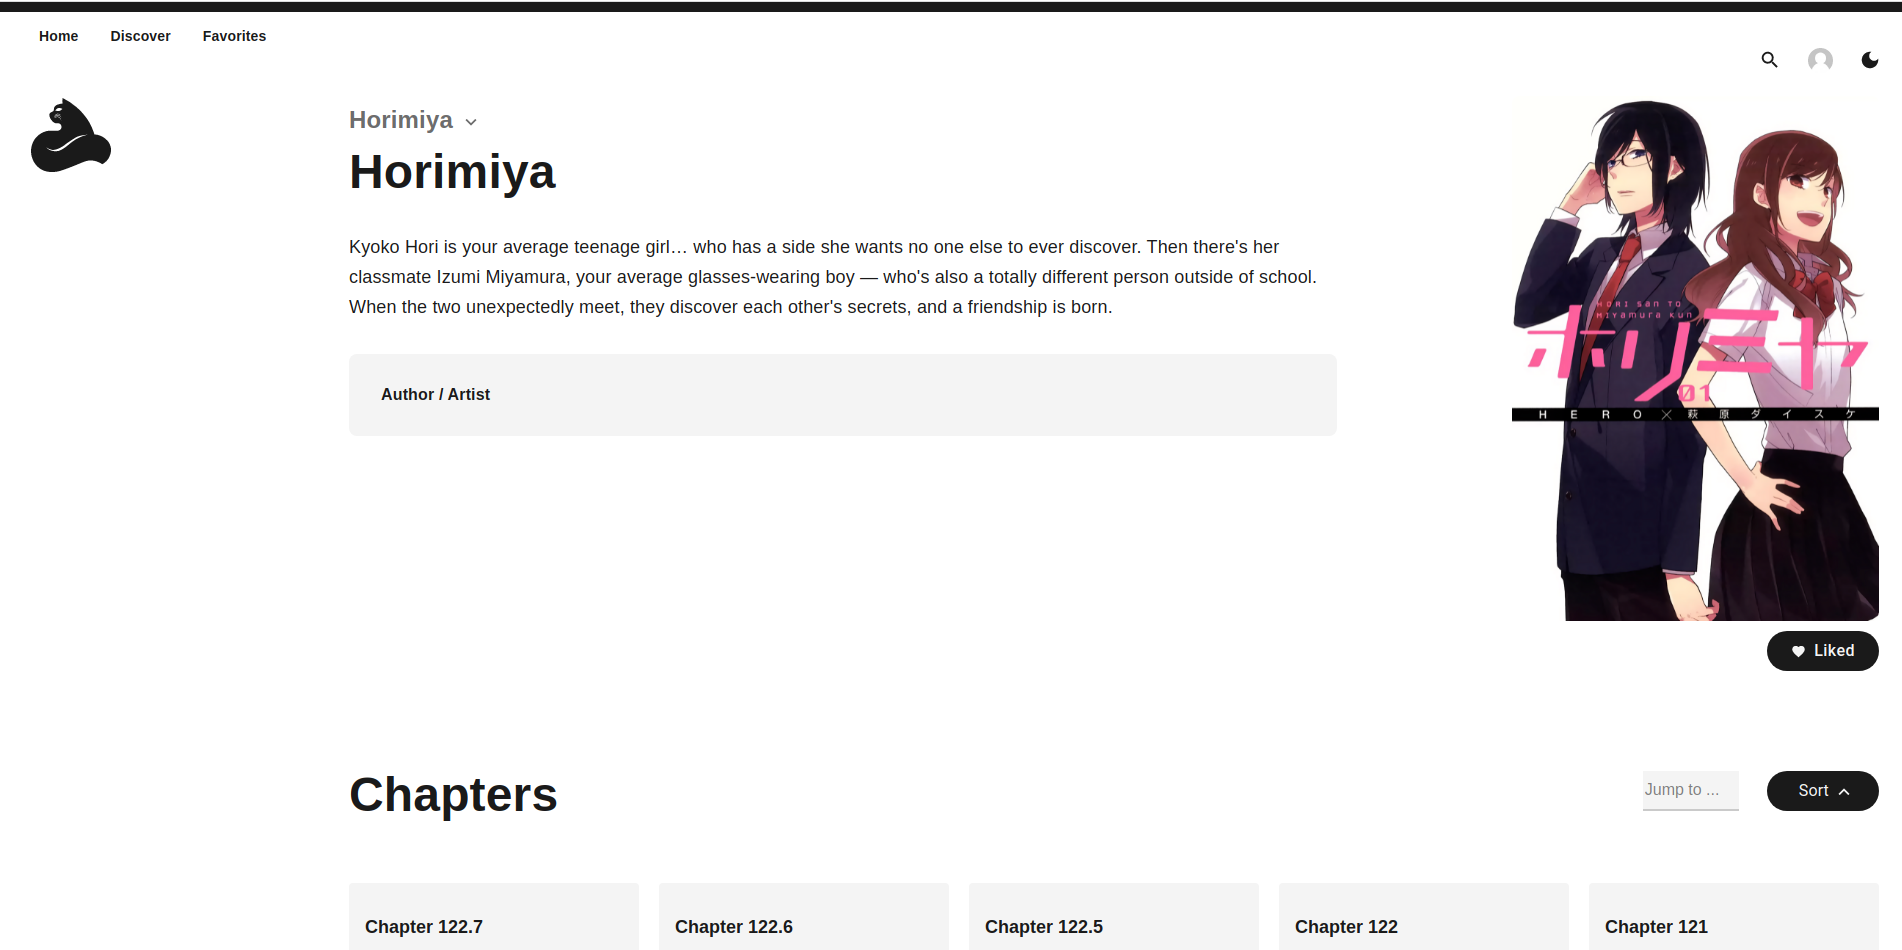
\includegraphics[width=\linewidth]{./images/image5.png}
	\caption{Màn hình đăng nhập}
	\label{fig:login_page}
\end{figure}

\subsubsection{Luồng sử dụng của sinh viên}

\paragraph*{Sinh viên đăng ký thực tập}

Tại màn hình trang chủ, sinh viên tìm kiếm công ty mà mình đang thực tập và đăng ký. Sau khi đăng ký thành công thì hệ thống sẽ thông báo lại như hình.

Hình \ref{fig:student_page} mô tả màn hình đăng ký thực tập của sinh viên.

\paragraph*{Sinh viên xem thông tin thực tập}
Sau khi đăng ký thực tập thành công, sinh viên vào kiểm tra thông tin thực tập của bản thân. Tại đây, sinh viên có thể xem thông tin công ty thực tập đã đúng chưa,  giảng viên hướng dẫn là ai, và nộp báo cáo.

Hình \ref{fig:view_internship_page} mô tả màn hình trang thông tin thực tập.

\begin{figure}[]
	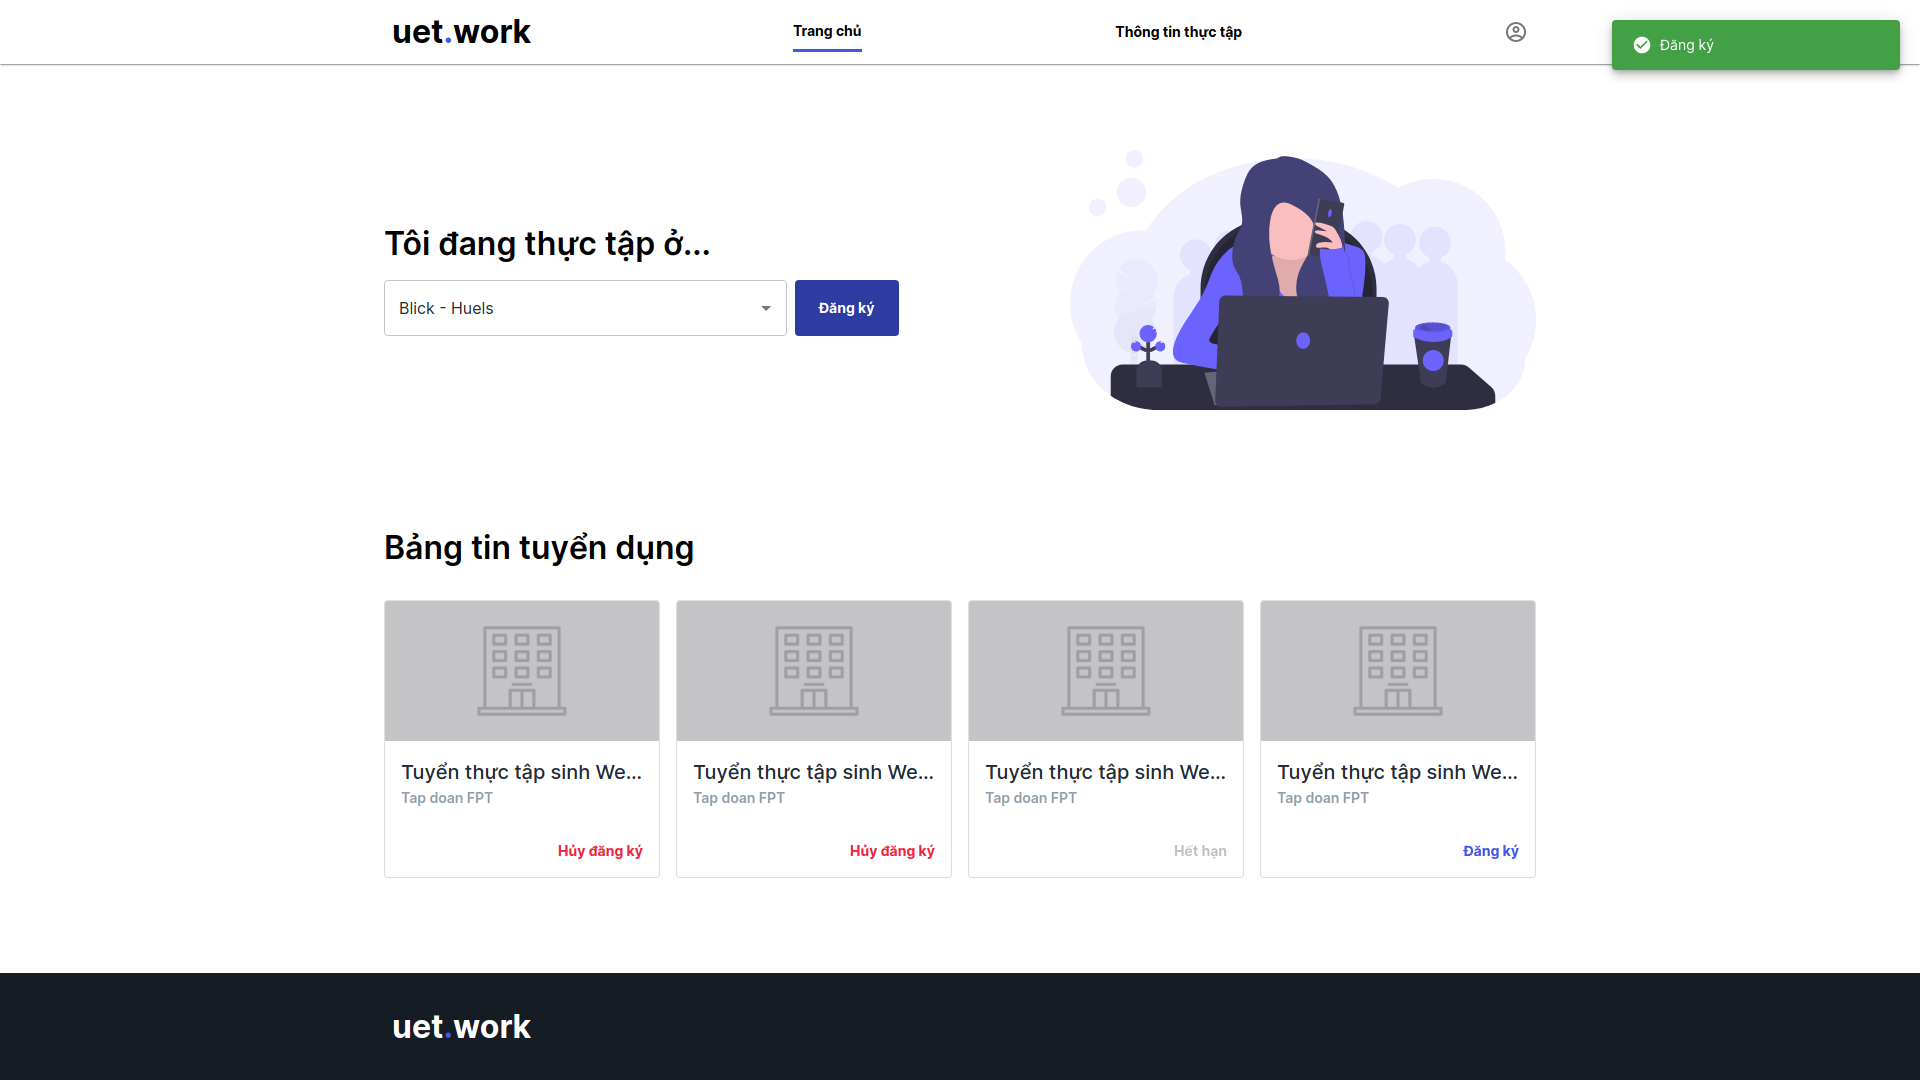
\includegraphics[width=\linewidth]{./images/image15.png}
	\caption{Sinh viên đăng ký thực tập}
	\label{fig:student_page}
\end{figure}

\begin{figure}[]
	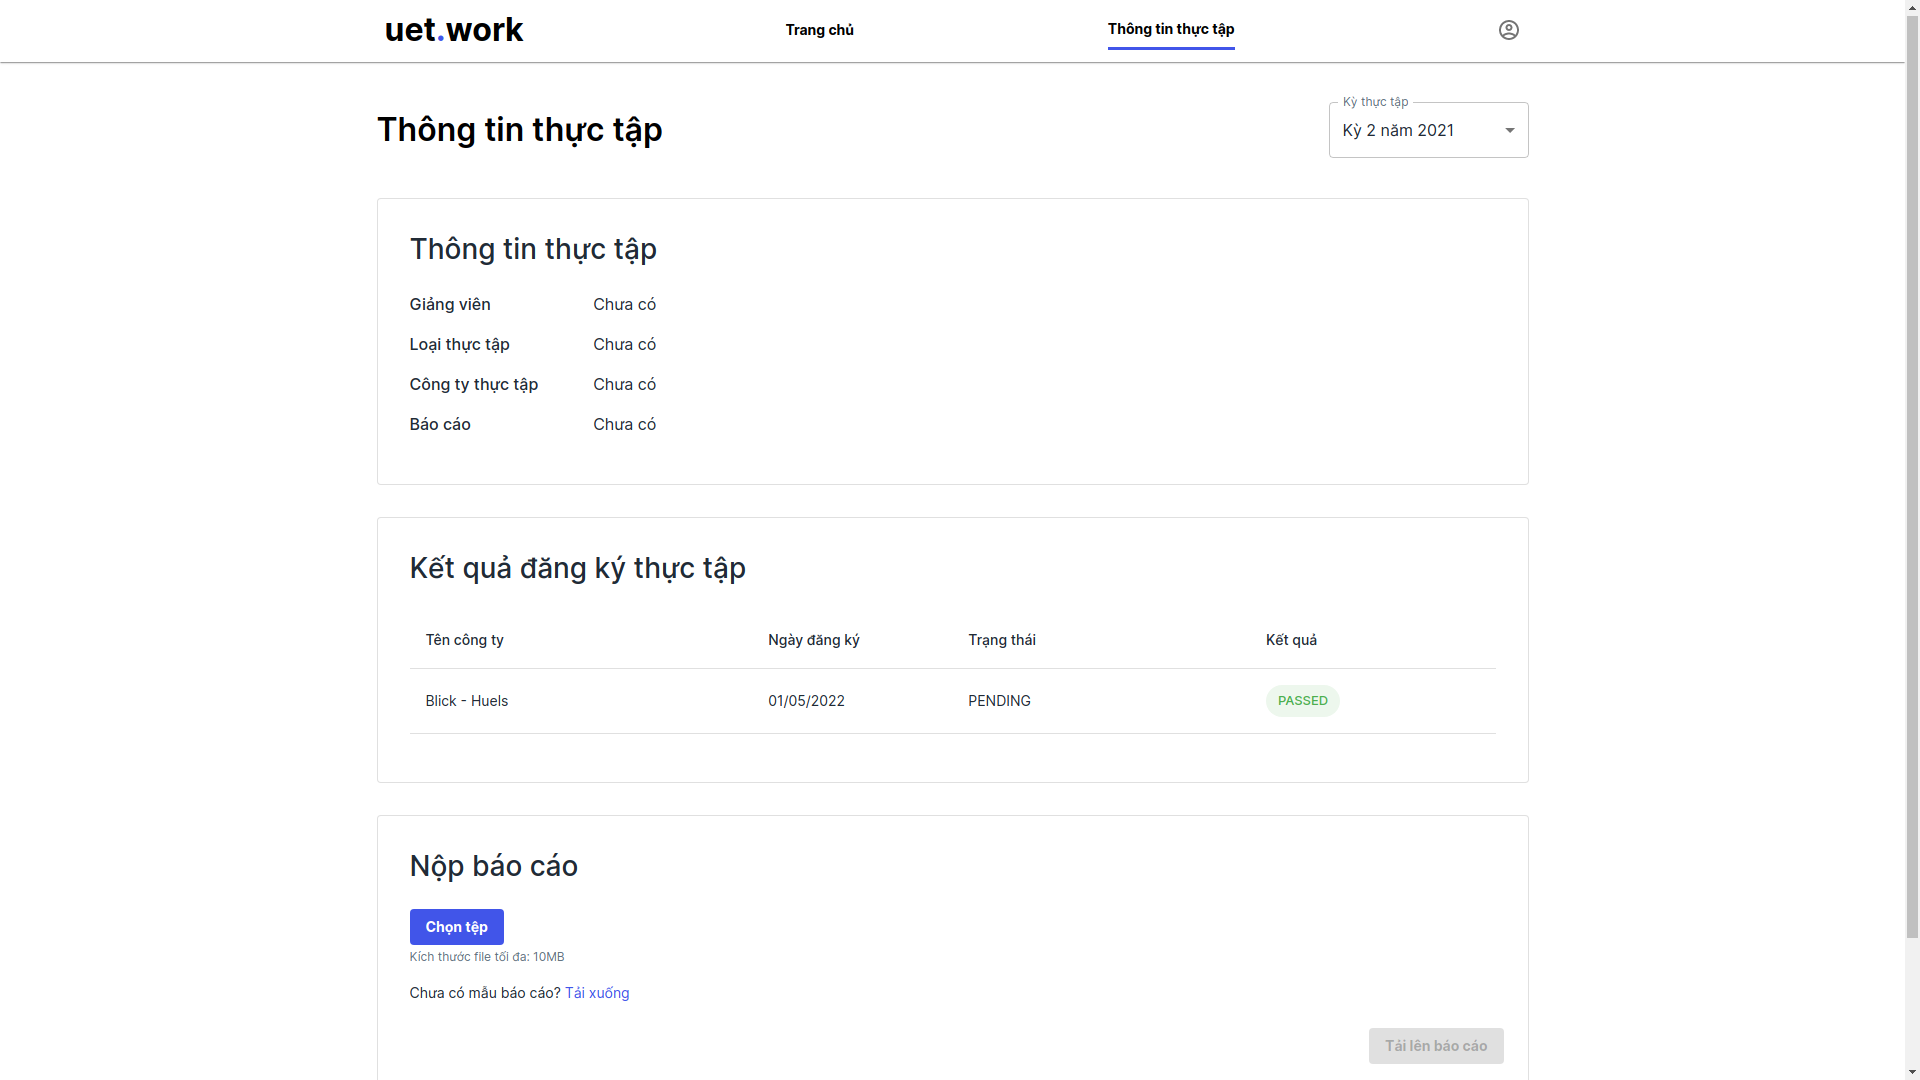
\includegraphics[width=\linewidth]{./images/image17.png}
	\caption{Sinh viên xem thông tin thực tập}
	\label{fig:view_internship_page}
\end{figure}

\subsubsection{Luồng sử dụng của giảng viên}

\paragraph*{Đọc báo cáo và chấm điểm cho sinh viên}

Tại đây, giảng viên tải xuống file báo cáo của sinh viên. Sau khi đọc và cho điểm xong, giảng viên thực hiện \emph{Thêm điểm} cho sinh viên.

Hình \ref{fig:working_student_page} mô tả màn hình danh sách sinh viên đang hướng dẫn.

\begin{figure}[]
	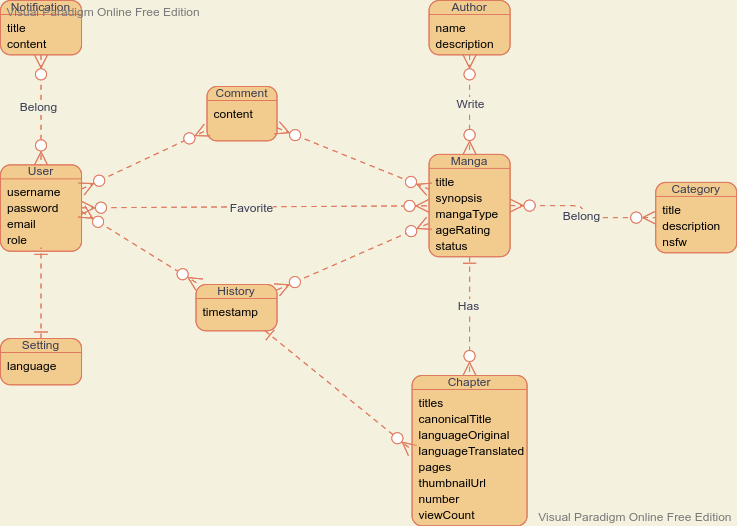
\includegraphics[width=\linewidth]{./images/image8.png}
	\caption{Màn hình danh sách sinh viên đang hướng dẫn}
	\label{fig:working_student_page}
\end{figure}

\subsubsection{Luồng sử dụng của đối tác}

\paragraph*{Thêm bài đăng tuyển dụng}

Tại trang Thêm bài đăng, đối tác thêm tiêu đề, nội dung chi tiết, số lượng tuyển dụng, ngày bắt đầu, ngày kết thúc, người liên hệ để tạo một bài đăng mới.

Hình \ref{fig:add_post_page} mô tả màn hình thêm bài đăng của đối tác.

\paragraph*{Chấp nhận / Từ chối yêu cầu thực tập}

Sau khi có các sinh viên đăng ký thực tập tại công ty, đối tác có thể vào trang Yêu cầu đăng ký thực tập để chấp nhận hoặc từ chối yêu cầu của sinh viên.

Hình \ref{fig:approve_or_reject_request} mô tả màn hình chấp nhận / từ chối yêu cầu thực tập.

\begin{figure}[]
	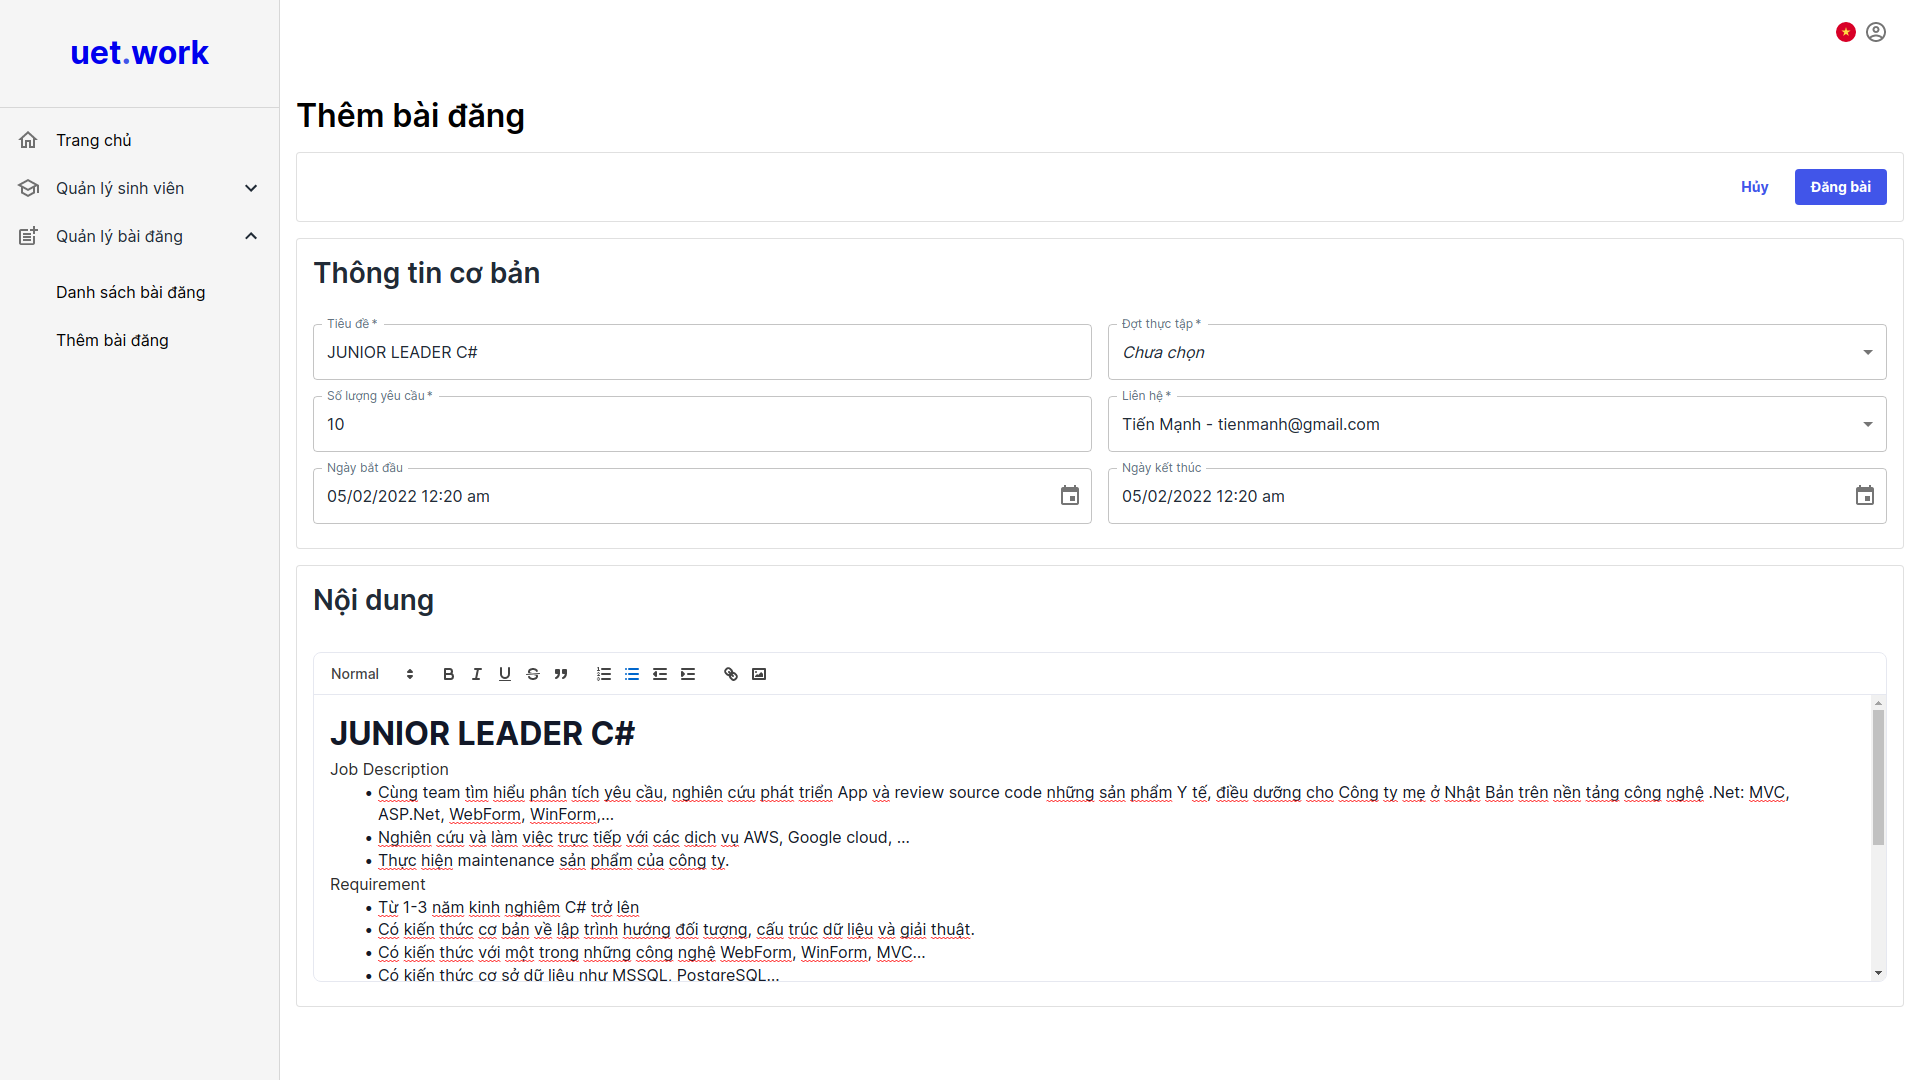
\includegraphics[width=\linewidth]{./images/image18.png}
	\caption{Màn hình thêm bài đăng mới}
	\label{fig:add_post_page}
\end{figure}

\begin{figure}[]
	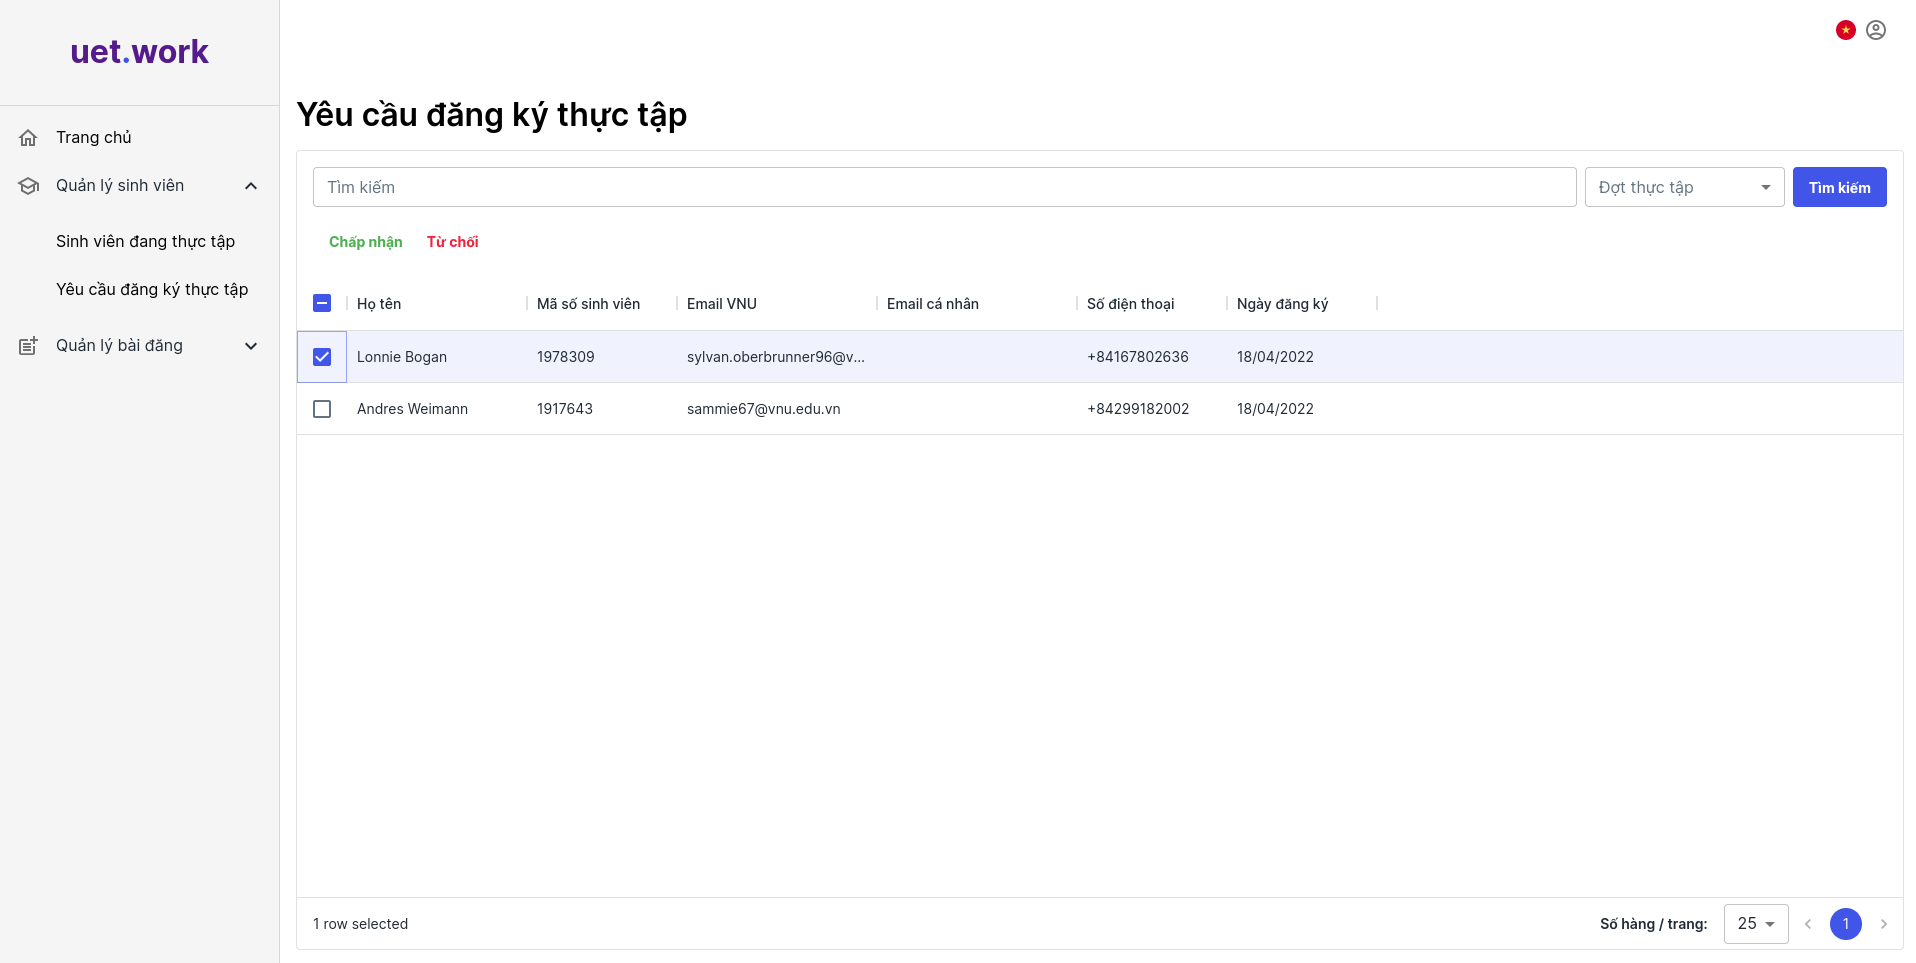
\includegraphics[width=\linewidth]{./images/image29.png}
	\caption{Màn hình chấp nhận / từ chối yêu cầu thực tập }
	\label{fig:approve_or_reject_request}
\end{figure}

\end{document}